\documentclass{report}
\usepackage[utf8]{inputenc}
\usepackage[english]{babel}
\usepackage[]{graphicx}
\graphicspath{ {Figures/} }
\usepackage{multirow}
\usepackage{enumitem}
\usepackage{tabularx}
\usepackage{booktabs}
\usepackage{ltablex}
\usepackage{amsmath}
\usepackage[parfill]{parskip}
% Set page margins
\usepackage[top=100pt,bottom=100pt,left=68pt,right=66pt]{geometry}
% Changes the style of chapter headings
\usepackage{titlesec}
\titleformat{\chapter}
   {\normalfont\LARGE\bfseries}{\thechapter.}{1em}{}
% Change distance between chapter header and text
\titlespacing{\chapter}{0pt}{50pt}{2\baselineskip}
\newcommand{\tabincell}[2]{\begin{tabular}{@{}#1@{}}#2\end{tabular}} 

\pagenumbering{roman}

\begin{document}
% Title
\begin{titlepage}
	\clearpage\thispagestyle{empty}
	\centering
	\vspace{1cm}

	% Titles
	% Information about the University
	{\normalsize The University of Melbourne \\ 
		School of Computing and Information Systems \\
		SWEN90016 Software Processes and Management\\
		Semester 1 – 2020 \par}
		\vspace{3cm}
	{\Huge \textbf{JJFresh -- Project Management Plan}} \\
	%\vspace{1cm}
	%{\large \textbf{xxxxx} \par}
	\vspace{3.5cm}
	{\normalsize Zhaofeng Qiu 1101584\\ % \\ specifies a new line
	             Chongjing Zhang 1055520\\
	             Pin Wang 1056745 \\
	             Yicun Tian 1088217 \\
	             Hongkang Li 977063\par}
	\vspace{3cm}
    
    \centering 
\includegraphics[scale=0.12]{logo.pdf}
    
    \vspace{0.5cm}
		
	% Set the date
	{\normalsize \today \par}
	\pagebreak
\end{titlepage}

\chapter*{Executive Summary}\label{sec:ESummary}
Jess and James plans to create an online store of fruits and vegetables as a JJFresh online sales platform for users to select and place orders. In this way, they want to maintain their existing customer base and remain competitive with other stores. In view of the insufficient budget of Jess and James, the students of registered software project management of the University of Melbourne are employed to develop this system. Based on the consideration of the changes in the needs of the project itself and the size of the development team, they chose an agile Scrum model, which will be assigned tasks to members by a short Sprint. They plan to deliver a product that meets core needs to Jess and James within 2 weeks, and complete 3 iterations of development within 4 weeks to deliver a complete website. The product will implement an online sales platform for Jess and James, thereby bringing them additional economic benefits. On the other hand, for the development team, the project will accumulate actual development experience, which will improve their competitiveness in future. 

\addcontentsline{toc}{chapter}{Executive Summary}
\pagebreak
\clearpage

\tableofcontents
\pagebreak

\chapter{Introduction}
\pagenumbering{arabic}
\section{Purpose of document}
   This document details how the development team plans, implements, and monitors the development of the JJFresh online store. According to the project requirements specification, this document describes in detail the scope of the project and possible risks, and how to control it. The development team also described the technologies that will be used throughout the development process. In addition, Scrum Master made a project plan for the development team's size and project needs. This document will serve as one of the true sources of all parties involved in the entire development cycle, such as Scrum Master, Product Owner and developers.

\section{Audience of document}
   All five people in the team participated in the preparation of the document. Firstly, Yicun Tian wrote the Executive Summary (part 2), Introduction (part 4), Roles and Responsibilities (part 6.1), Communication Plan (part 6.2) and Risk management (part 6.3) of the document.Secondly,Hongzhang Li completed Project Information (part 5). Moreover, Pin Wang and Chongjing Zhang as developers completed Technology (part 6.4). Zhangfeng Qiu, who served as Scrum Master, completed the Project Planning (6.5) and final proofreading of all document.

\section{Evolution of document}
\begin{tabularx}{0.95\linewidth}{%
  l%
  >{\raggedright\arraybackslash}p{2.2cm}%
  >{\raggedright\arraybackslash}p{1.5cm}%
  >{\raggedright\arraybackslash}X}
  \toprule
  Version & Created by & Date created & Comments\\
  \midrule
  Version 1.0
  & Yicun Tian, Hongkang Li, Pin Wang, Chongjing Zhang, Zhangfeng Qiu
  & 4.27
  & In this version, five people of the team cooperated to complete section 1 to 6 of the Project Management Plan. In this process, we mainly carried out the preparation work before development, including the definition of key stakeholders, Scope and SDLC of the project, evaluation of business value, constraints, the definition of people's role in the team, communication plan, risk management, definition of the technology used in the project and project planning.
  % \\
  % \midrule
  % Version 1.1
  % & 
  % & 5.23
  % & 
  % \\
  % \midrule
  % Version 1.2
  % &
  % & 5.30
  % &
  % \\
  % \midrule
  % Version 1.3
  % & 
  % & 6.5
  % & 
  \\
  \bottomrule
  \\
  \caption{Evolution of document}  
  \label{tab:evolutionOfDocument}
\end{tabularx}

%%%%%%%%%%%%%%%%%%%%%%%%%%%%%%%%%%%%%%%%%%%%%%%%%%%%
\chapter{Project Information}
\section{Key Stakeholders}
\begin{tabularx}{0.95\linewidth}{%
  >{\raggedright\arraybackslash}l%
  >{\raggedright\arraybackslash}p{1.5cm}%
  >{\raggedright\arraybackslash}X}
  \toprule
  Stakeholders & Internal/ External & Influence on Project \\
  \midrule
  Jess and James
  & Internal
  & Jess and James are the people who defined the requirements of the project. They will not directly participate in the development of the online store website. They are users of the website and can provide feedback to the development team during the development process.
  \\
  \midrule
  The teaching team
  & Internal
  & The teaching team of SWEN90016 is playing the role of Product Owner in the project. They are responsible for contact with Jess and James and understand their need.  They cooperate with the SCRUM master of the project and help define the product backlog. Also, they give advice and feedback to the student team during the development process.
  \\
  \midrule
  The student team
  & Internal
  & The student team cooperates as a SCRUM team in the project. They are responsible for both planning and developing the online store project. 
  \\
  \midrule
  Customers
  & External
  & The satisfaction of the customers is an important factor for project success. The main source of website revenue comes from them. Their feedback can help the development team improve the application.
  \\
  \bottomrule
  \\
  \caption{Stakeholder Register}  
  \label{tab:stakeholderRegister}
\end{tabularx}

\section{Scope}
\subsection{What is in-scope?}
\begin{enumerate}
  \item Login system: User need to register an account with personal information (name, phone number, email, address etc.) when the first-time use. They can login to the online store website after registration by inputting their username and password.
  
  High priority: Online store website is not for browsing information, it is the platform for trading fruits and vegetables. Every user will purchase products through their account, which is the basic function of this online store website.

  \item Management of personal information: User can add or edit their personal information. For example, if they change their phone number or move to the new house, updating the personal information will be the necessary.
  
  High priority: If the customers change their phone number or address, this function is important to avoid some trouble caused by information asymmetry. For example, Jess and James may delivery products to the wrong address and cannot contact buyer.
  
  \item Commodity display system: Website should display all type of the products with different size and price to the users whenever they are going to purchase or just browse it.
  
  High priority: User should know which products are sold in this online store and its size and price. Purchase cannot be made without this function because customers do not even know which fruit and vegetable they can buy.
  
  \item Order processing system: User can place their orders after selecting what they want. They can also change or cancel their orders. Jess and James can management these orders in the website background.
  
  High priority: It is the basic part of the purchase function. Online store cannot do any business without orders.
  
  \item Message confirmation function: After placing the orders, Jess and James will deal with the orders. If the orders are confirmed, a message will be sent to the users to let they know their orders are confirmed.
  
  High priority: Confirmation system is the important part in the business online. If the customers place the order while the store owner ignore it, they will never know whether their orders are confirmed or not without confirmation message system.
  
  \item A database which can store user account, order list, product information.
  
  High priority: Online store is a type of software products which need database to store more and more data.
  
  \item Date selecting function: In this project, customer should be able to choose a day and time for delivery.
  
  High priority: Because JJFresh online store offer delivery service, the date selecting system is the important part of delivery.
\end{enumerate}
\subsection{What is out-of-scope?}
The future enhancements are out-of-scope
\begin{enumerate}
  \item Online payment system.
  \item Navigation system on delivery.
\end{enumerate}
The following are more out-of-scope
\begin{enumerate}
  \item Distance judgment function. Jess and James should determine the distance between courier destination and JJFresh within 10km by themselves.
  \item Communication service with customers except confirmation message sending. Jess and James decide how to communicate with their users when necessary, such as call or email to him/her.
\end{enumerate}
%%%%%%%%%%%%%%%%%%%%%%%%%%%%%%%%%%%%%%%%%%%%%%%%%%%%%
\section{Delivery approach}
The delivery approach we choose for our project is \textbf{SCRUM}, an agile method that can provide high flexibility and quick delivery. Our decision is based on the following reasons.
\begin{enumerate}
  \item Scrum can provide an incremental delivery system to help the JJFresh online store retain flexibility while continually producing outcomes. As each sprint backlog represents a new release of the product, we can shorten the time for the project to our clients and improve the user experience of the website based on the feedback from them. Clients are continuously involved during every stage. And it can reduce waste and rework and increase the satisfaction of clients.
  \item The sprint process in the SCRUM model can provide regular adaptation to changing circumstances. Unlike the Waterfall model, which is very difficult to move back to makes changes in the previous phases, using Scrum would make the development of the JJFresh online store website able to adapt to unforeseen circumstances, allowing for changes to be easily incorporated if required.
  \item By doing sprint review and sprint retrospective at the end of each sprint, the client and team know exactly what is complete and what is not. This reduces the risk in the development process.
  \item SCRUM intends small or mid-sized dedicated teams with high coordination, which is suitable for our team with five members. The Waterfall model, which involves large teams and lack of coordination among team members, can not meet our needs.
\end{enumerate}
%%%%%%%%%%%%%%%%%%%%%%%%%%%%%%%%%%%%%%%%%%%%%%%%%%%%%
\section{Business Value}
JJFresh is currently busy in the morning but almost empty in the afternoon. The deployment of this project will keep JJFresh's existing customers who shop in the morning and shift the afternoon business hours from offline to online, which offers delivery service for current and potential customers who cannot go to JJFresh store at that time. The online store will operate 24 / 7, which is much longer compare to the old business hours, thus provides customers with the convenience of placing orders at any time. With these advantages, the online store project would attack more customers for JJFresh. The increase in customers can increase fruit and vegetable orders, and therefore help Jess and James gain more financial benefits and avoid JJFresh from being closed. The financial and Non-Financial benefits for different stakeholders are shown in Table \ref{tab:businessValue}.

\begin{tabularx}{0.95\linewidth}{%
  >{\raggedright\arraybackslash}l%
  >{\raggedright\arraybackslash}X%
  >{\raggedright\arraybackslash}X}
  \toprule
  Stakeholders & Financial benefits & Non-Financial Benefits \\
  \midrule
  Jess and James
  & Jess and James are the business owners of the JJFresh online store project. The success of the project can help them change their business model. They would gain more customers due to the extension of the business model. Also, the increase in customers would increase the number of orders, which can increase their revenue.
  & They can gain experience in operating an online fruit shop. The online store website can also increase the chance of JJFresh being searched by a search engine of a browser, which can improve the exposure, thereby improving their brand awareness. 
  \\
  \midrule
  The teaching team
  & The teaching team of the Software Processes and Management subject is employed by the school. They can get salary by guiding students.
  & Teaching students in this project can increase their experience in teaching and management.
  \\
  \midrule
  The student team
  & If the project achieves commercial success, students may receive financial awards from Jess and James.
  & They would gain software development experience from the project, which can increase their project experience and help boost their CV. Also, working as a team can improve their teamwork ability.
  \\
  \midrule
  Customers
  & For the customers who are used to buy fruits from JJFresh, home delivery can save them time and money. They don't need to spend money on transportation to jjfresh. Of course, the delivery fee must be considered. But it would be a trade-off.
  & Customers would be able to buy fruits and vegetables with high quality in a more convenient way. Also, for unforeseen circumstances like Covid-19, buying online can reduce their unnecessary travel and keep them safe.
  \\
  \bottomrule
  \\
  \caption{Business Value}  
  \label{tab:businessValue}
\end{tabularx}
%%%%%%%%%%%%%%%%%%%%%%%%%%%%%%%%%%%%%%%%%%%%%%%%%%%%%
\section{Constraints}
\begin{itemize}
  \item Team members are lack of experience in SCRUM. SCRUM is an Agile process and is difficult to do without experience, especially an experienced SCRUM master. The student who plays the role of SCRUM master has no SCRUM management experience before. There may be many problems during the development process.
  \item People in the development team are unfamiliar with creating a website in Wix.com. Also, students who are responsible for the implementation of the project are not full-time workers. The efficiency of their development may be low, which may result in the delay of the project.
  \item A virtual team may not able to follow all the processes in SCRUM. Appropriate improvements and compromises would be applied to some specific processes in the SCRUM. Communication in a virtual team is less frequent and less rich than face-to-face interaction. Some of the team members are not in Australia, and because of the time difference, daily SCRUM will be conducted via chat, which may bring negative effects to the project.
  \item The tool provided by Wix.com only has limited functions, which make it impossible to achieve the requirements perfectly. And the website implement by Wix.com has poor scalability. If Jess and James want to expand their business scale, the development team may have to redevelop the entire project with other web technics.
  \item The delivery range of Jess and James is limited, and users who are too far away cannot get services.
  \item The time limit of the project is only about one month. The overall implementation of the project may not be perfect in such a short time.
\end{itemize}
%%%%%%%%%%%%%%%%%%%%%%%%%%%%%%%%%%%%%%%%%%%%%%%%%%%%%

\chapter{Project Governance}
\section{Roles and Responsibilities}
\begin{tabularx}{0.95\linewidth}{%
  l%
  >{\raggedright\arraybackslash}p{2.2cm}%
  >{\raggedright\arraybackslash}X}
  \toprule
  Roles & Member & Responsibilities \\
  \midrule
  Scrum Master
  & Zhangfeng Qiu
  & The Scrum Master is the person in charge of the process. His main responsibility is to guide the development team and product owners in daily development activities.
  \\
  \midrule
  Product Owner
  & Jess and James, Tutors
  & The product owner is the spokesperson for the customer or stakeholders. Their main responsibility is to ensure that product to-do items are transparent and clearly expressed, and everyone in the team has the same understanding of the project.
  \\
  \midrule
  Dev Team Members
  & Pin Wang, Chongjing Zhang
  & The Scrum development team is composed of professionals who deliver the incremental work of "Done" products that may be released at the end of each Sprint
  \\
  \midrule
  Subject Matter Expert
  & Tutors, Tian Yicun, Li Hongkang
  & Somebody with specialized knowledge or talent that is needed by the Team
  \\
  \bottomrule
  \\
  \caption{Roles and Responsibilitiest}  
  \label{tab:rolesResponsibilities}
\end{tabularx}

\section{Communication Plan}
Our group first uses “slack” for the main information transfer, such as publishing message notifications, file sharing, etc. Secondly, using “trello” to arrange the various stages of the project plan and the content is managed by the scrum master. Furthermore, “github” is used to manage output products, such as the release of code and report.

According to the scrum development cycle and the difficulty of this project development, we will conduct a 15-minute meeting discussion on zoom every day, mainly to summarize the results of yesterday and the arrangement of today's tasks. If a team member is absent from a meeting, the person in charge will use email or telephone to communicate with him.

\section{Risk Management}
\subsection{Risk Impact Analysis Table}
\begin{tabularx}{0.95\linewidth}{%
  >{\raggedright\arraybackslash}p{1cm}%
  l%
  >{\raggedright\arraybackslash}p{2cm}%
  l
  >{\raggedright\arraybackslash}X%
  >{\raggedright\arraybackslash}X}
  \toprule
  Risk ID & Risk Type & Description & Probability & Impact & Justification\\
  \midrule
  1
  & Project
  & The software developed by wix has low scalability.
  &
  &
  &
  \\
  \midrule
  2
  & Business
  & Jess and James cannot deliver in time due to unforeseen circumstances.
  &
  & If Jess and James cannot deliver the order because of the coronavirus, the economic loss is relatively small.Because the number of orders during the coronavirus will also decrease. However, if one of them is sick and the manpower is insufficient, the order cannot be delivered or the delivery is not timely, which will cause the customer to refund the order and bring them huge economic losses. Even they may lose customer expectations and trust.
  & Because of the current coronavirus, when the condition is serious, Jess and James cannot deliver the product to the door. Considering that only two people, Jess and James, are currently packaging and distributing all orders, when one of them is sick, it is impossible to deliver fruits and vegetables.
  \\
  \midrule
  3
  & Business
  & Cancel orders maliciously or for no reason.
  &
  & The user can cancel the order on the day of product delivery or cancel the agreed order after the seller purchases the goods. These cancellations are unreasonable or caused by the buyer ’s own reasons, but these actions will cause the seller to accumulate vegetables and fruits and waste time and human resources.
  & The buyer may cancel the order for many reasons, but the consequences of this risk need to be borne by the buyer. For example, the buyer may cancel the order because the amount of vegetables and fruits is too large, but it is no longer needed or it is considered more cost-effective. These actions will lead to the occurrence of this risk.
  \\
  \midrule
  4
  & Business
  & Buyer declares that there is a problem with the quality of the product received.
  &
  & The buyer believes that the fruit or vegetable received is not fresh, or the size, softness do not meet expectations, resulting in a refund and economic loss to the buyer.
  & Because the buyer buys the product according to the pictures and descriptions on the website and does not see the real thing. However, if the seller uploads a virtual picture or picks the best of vegetables and fruits to take a picture, it will result in inconsistency between the items received by the buyer and the picture. As a result, buyers do not recognize the product quality and refund the order.
  \\
  \midrule
  5
  & Project
  & User cannot receive email in time.
  &
  & When the buyer is unable to receive the feedback email in time, the buyer is not sure whether the order has been placed or cancelled successfully. It may cause the buyer to repeat the operation and bring losses to the buyer or seller. Eventually, the user's sense of experience is reduced. For example, a buyer who repeats a booking without receiving an email after ordering a product may cause the buyer to receive 2 copies of the same product and pay an additional fee.
  & If the network conditions of the buyer or the seller are poor, the network is actually delayed, resulting in the buyer not being able to receive the email immediately after performing the operation. At the same time, if there is a problem due to the system's automatic mail reply function, it will also cause the user to not receive the mail.
  \\
  \bottomrule
  \\
  \caption{Risk Impact Analysis Table}  
  \label{tab:riskImpactAnalysisTable}
\end{tabularx}

\clearpage
\subsection{Risk Register}
\begin{tabularx}{0.95\linewidth}{%
  >{\raggedright\arraybackslash}p{1cm}%
  >{\raggedright\arraybackslash}p{2cm}%
  >{\raggedright\arraybackslash}p{2cm}%
  >{\raggedright\arraybackslash}X%
  >{\raggedright\arraybackslash}p{2cm}%
  >{\raggedright\arraybackslash}p{2cm}}
  \toprule
  Risk ID & Trigger & Owner & Response & Response Strategy Type & Resources Required\\
  \midrule
  1
  &
  & 
  &
  &
  &
  \\
  \midrule
  2
  & The seller is sick or the coronavirus is serious
  & Jess and James
  & If the coronavirus should affect the delivery, the buyer needs to cancel the order. If the order cannot be delivered in time because the seller is sick or other assents, they can hire another person to deliver. 
  & Mitigate/accept
  & 
  \\
  \midrule
  3
  & A user repeatedly cancels an order without reason, or the user cancels a large order
  & Jess and James
  & For example, by limiting the number of orders that the user cancels per week or limiting the time when the user cancels the order. Failure to cancel the order within the first 24 hours of the specified delivery time would be a viable solution. For a large number of orders, the seller should require the buyer to advance a part of the deposit in order to make up for the economic loss after canceling the order.
  & Mitigate
  &
  \\
  \midrule
  4
  & The seller's feedback after receiving the product
  & Jess and James
  & The chat function can be opened in the software, so that the buyer can leave a message to the seller through the chat box. For example, the kiwi fruit that the buyer wants to get is hard and can be stored for at least 2 days. At the same time, buyers can also use the chat function to provide sellers with videos and photos of vegetables and fruits.
  & Mitigate
  &
  \\
  \midrule
  5
  & User cannot receive mail
  & users or developers
  & If this risk occurs due to network extension, the system should be able to automatically detect the user's network conditions and promptly prompt. For example, when the buyer's network conditions are poor, the system should prompt the user that the operation may not be successful when the user submits the order or cancels the order. If the email is not received in time, please contact the seller to check whether the operation is successful. If there is a problem with the function of auto-replying emails, the administrator of the maintenance system should be able to detect it in the background, the system is abnormal, and fix the bug in time.
  & Mitigate
  &
  \\
  \bottomrule
  \\
  \caption{Risk Register}  
  \label{tab:riskRegister}
\end{tabularx}

\section{Technology}
\section{Project Planning}
The SDLC of our project is SCRUM. Since the key requirements for the initial development provided by Jess and James are fixed, a Fixed-Scope Release Planning would be used to plan our project.

\subsection{Product Backlog}
The detail of product backlog is shown in table \ref{tab:productBacklog}. BFTB Score is the abbreviate of the Bang-for-the-Buck Score, which is a way of measuring how to get the most value in the shortest time. It is used to help assess the priority of the features. The BFTB Score is calculated by the formula below:
$$
  \text{BFTB Score} = \frac{\text{Value Point}}{\text{Store Point}}
$$

The story points of different features are estimated by the development team and the SCRUM master, based on the volume, risk, uncertainty and complexity of the features. The value points of them are estimated by the product owners. \textbf{Fabonacci sequence} is used to provided relative estimation to both story point and value point. Each story point equals about an hour of work.

Except for the tree future user stories at the end of the product backlog table, all others are must-have stories because they are key requirements defined by Jess and James.
\begin{tabularx}{0.95\linewidth}{%
  >{\raggedright\arraybackslash}p{1.5cm}%
  >{\raggedright\arraybackslash}X%
  >{\raggedright\arraybackslash}X%
  p{1cm}p{1cm}p{1cm}
  }
  \toprule
  Feature & User Story & Tasks & Story Point & Value Point & BFTB Score\\
  \midrule
  Browse product menu 
  & As a customer, I want a menu that shows all the products, so that I can know what products are the website selling. 
  & 1.Provide a page for showing the list of the products\textit{(3-hour)}; 2.Show the types of the products\textit{(1-hour)}; 3.Show the price of the products\textit{(1-hour)}; 4.The price would change automatically\textit{(1-hour)}; 5.Show the pictures of products\textit{(1-hour)}.
  & 8
  & 5
  & 0.625
  \\
  \midrule
  Customer sign up
  & As customers, I want to sign up for the website, so that I can a member of the website.
  & 1.Check whether the information of the user is valid\textit{(1-hour)}; 2.Add the user to the database and send a confirming email to the new member if valid\textit{(1-hour)}.
  & 2
  & 2
  & 1
  \\
  \midrule
  Customer sign in and sign out
  & As customers, I should be able to sign in and sign out, so that I can manage my account and orders.
  & 1.Sign in, check whether the user exist and whether the user's password correct\textit{(1-hour)}; 2.Sign out\textit{(1-hour)}; 3.Handle the problem of forgetting the user password (Allow password reset)\textit{(1-hour)}.
  & 3
  & 3
  & 1
  \\
  \midrule
  Customer add and edit client information
  & As customers, after login, I can add or edit my information like home address, user name, email address, and contact number.
  & 1.Add and edit the name, email address, home address\textit{(1-hour)}; 2.Add and edit up to three multiple contact phone numbers\textit{(1-hour)}.
  & 2
  & 3
  & 1.5
  \\
  \midrule
  Add products to shopping cart
  & As customers, after login, I can add or edit my information like home address, user name, email address, and contact number.
  & 1.Select size, type and amount of the products and add them to shopping cart.\textit{(2-hour)}
  & 2
  & 5
  & 2.5
  \\
  \midrule
  Manage shopping cart
  & As a customer, I want to manage my shopping cart, so that I can remove those I don't want or add some more products.
  & 1.Select the items to pay\textit{(1-hour)}; 2.Change the amount of items\textit{(1-hour)}; 3.Delete items\textit{(1-hour)}; 4.View the price of the items selected\textit{(1-hour)}; 5.Provide a page to show all the items in the shopping cart\textit{(3-hour)}.
  & 8
  & 5
  & 0.625
  \\
  \midrule
  Check out shopping cart
  & As a customer, I want to choose the day and time for delivery, so that I can get the fruit on the right day.
  & 1.Choose a day and time for delivery.\textit{(1-hour)}. Only two bookings are allowed in a particular-hour.); 2.Send a confirming email to the customer\textit{(1-hour)}; 3.Show the day and time which is valid\textit{(2-hour)}; 4.Add an order to the user's order list\textit{(1-hour)}; 5.Handle synchronization problem\textit{(2-hour)}.
  & 8
  & 5
  & 0.625
  \\
  \midrule
  Cancel orders
  & As a customer, I need to get the ability to cancel an order so that I can modify an order and then re-create.
  & 1.Cancel order\textit{(1-hour)}; 2.Send emails to both customer and admin\textit{(1-hour)}.
  & 2
  & 2
  & 1
  \\
  \midrule
  Build database
  & As an admin, I need a database, so that I can store all the information of customers orders.
  & 1.Define the order model\textit{(1-hour)}; 2.Define the user information model\textit{(1-hour)}; 3.Define the admin information model\textit{(1-hour)}; 4.Create table and relation\textit{(2-hour)}; 5.Test\textit{(1-hour)}
  & 8
  & 5
  & 0.625
  \\
  \midrule
  Admin sign in and sign out
  & As an admin, I want to provide my username and password, so that I can register an admin account.
  & 1.Sign in\textit{(1-hour)}; 2. Sign out\textit{(1-hour)}.
  & 2
  & 2
  & 1
  \\
  \midrule
  View and manage orders
  & As an admin, I want the specific information of the user's order, so that I can packaging user orders.
  & 1.Confirm order\textit{(1-hour)}; 2.Order rank by date\textit{(1-hour)}; 3.Cancel order and provide reason\textit{(1-hour)}; 4.Provide a page to show order list with order information attach to it\textit{(4-hour)};
  & 8
  & 5
  & 0.625
  \\
  \midrule
  Manage product infomation
  & As an admin, I want to manage product information, so that I can change the price or picture of my products.
  & 1.Change the price of products\textit{(1-hour)}; 2.Change the pictures of products\textit{(1-hour)}; 3.Change the type of products\textit{(1-hour)}; 4.Add products\textit{(1-hour)}; 5.Delete products\textit{(1-hour)}.
  & 5
  & 3
  & 0.6
  \\
  \midrule
  Register admin account
  & As an admin, I need to get the ability to register for a new admin account, so that I can get more admin accounts if I need them.
  & 1.Provide way for admin account registration\textit{(1-hour)}.
  & 1
  & 1
  & 1
  \\
  \midrule
  Edit admin account information
  & As an admin, I may want to edit my admin account information, so that I can change the password.
  & 1.Provide way for admin account information editing\textit{(1-hour)}.
  & 1
  & 1
  & 1
  \\
  \midrule
  Add multiple bookings for the same slot
  & As an admin, I want to add multiple bookings for the same slot in the future. So that I  can employ others to deliver boxes.
  & 1.Allow multiple bookings for the same slot\textit{(6-hour)}.
  & 8
  & 2
  & 0.25
  \\
  \midrule
  Using AI to calculate delivery routes and times
  & As an admin, I want to use AI technology to help me calculate an optimal route and time for delivery.
  & 1.Create a model and an algorithm for the AI to learn and help calculate the optimal routes and time for delivery\textit{(12-hour)}.
  & 13
  & 3
  & 0.231
  \\
  \midrule
  Extended to allow for payment online.
  & As an admin, I want to be paid online, so that I can save my time and improve the delivery efficiency.
  & 1.Provide ways for online payment\textit{(5-hour)}; 2.Secure user information\textit{(8-hour)}.
  & 13
  & 3
  & 0.231
  \\
  \bottomrule
  \\
  \caption{Product Backlog}  
  \label{tab:productBacklog}
\end{tabularx}  

\subsection{Must-have Story Points}
Without calculating the features needed in the future, the total number of must-have story points is 60.
$$
SP_{total} = 60 \text{ (Story Point)}
$$

\subsection{Velocity Estimating}
There are two developers in our team. Since both of them are students, each of them can only spend about 1.2 to 1.5 hours a day on the project. They can work five days a week, so the total working hours of a week are 12 to 15 hours. We expect each story point to be equivalent to one hour of working time. So the min velocity ($V_{min}$) for a two-week sprint is about 24 story points, and the max velocity ($V_{max}$) is about 30 story points. And by using the formula shown below, we can get our minimum and maximum number of sprints, which are 2 and 2.5, respectively. The inital burndown chart for the whole project is shown on figure \ref{fig:burndown1}.
$$
S_{min} = \frac{SP_{total}}{V_{max}}
\text{, } 
S_{max} = \frac{SP_{total}}{V_{min}}
$$
\begin{figure}[htp]
\centering
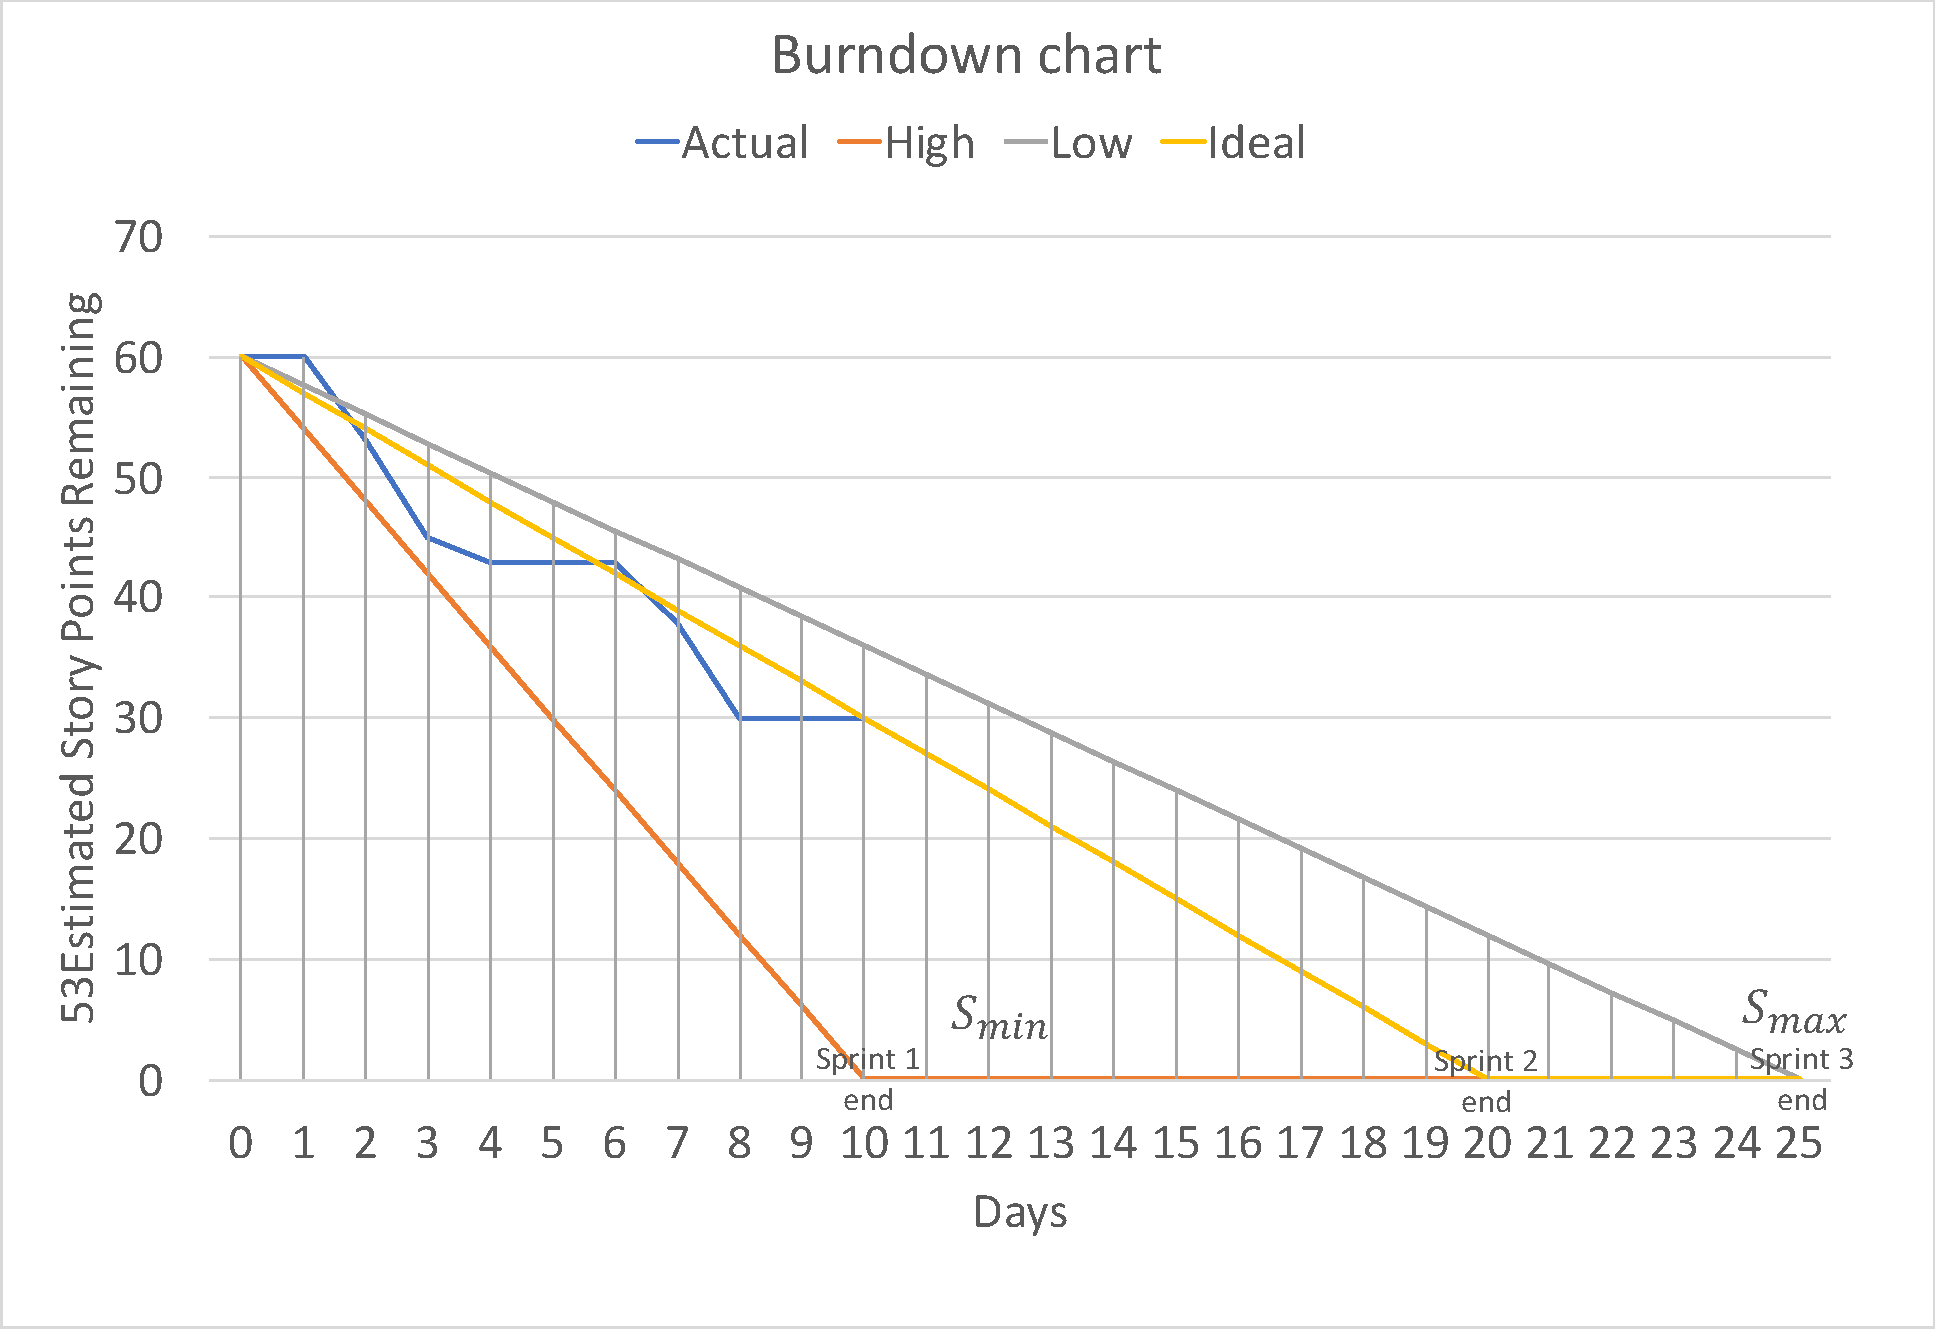
\includegraphics[width=\textwidth]{Figures/burndown1.pdf}
\caption{Initial Burndown Chart for the Whole Project}
\label{fig:burndown1}
\end{figure}

\subsection{Sprint Planning}
\subsubsection{Sprint Cycle}
\label{sec:sprintCycle}
The development phase of our project would start on \textbf{Monday, April 25}. Since the final delivery due date of the whole project is \textbf{June 1}, we decided to divide our development into three phases, each corresponding to a sprint.

The first phase is to let the website go online without the function of purchase. The website can display all kinds of information about the products and provide the service of user registration. At the same time, the database is initially established to record the data of users and products. The first sprint will last for two weeks, \textbf{from Monday, April 27 to Friday, May 8}. 


In the second phase, we need to realize the function that users place orders to purchase products, and sellers can view and modify user orders. Preliminary testing will also take place at this phase. The second sprint will last for two weeks, \textbf{from Monday, May 11 to Friday, May 22}.

The third stage is mainly based on user feedback to repair the vulnerability, carry out more tests and improve the existing functions. If some functions left over from the first two sprints are not implemented, they will also be solved in this sprint. As the project is nearing its end and there is less work left, the sprint in this phase will last only one week, \textbf{from Monday, May 25 to Friday, May 29.}

On \textbf{the first Monday of every sprint}, a Sprint Planning meeting would be held to select high priority items from the product backlog that the development team can commit to delivering in a single Sprint. The select itmes would be add to Sprint Backlog.

On \textbf{the last Friday of each sprint}, a Sprint Review meeting would be held to demonstrate the new features to Stakeholders, and a Sprint Retrospective meeting would be held to review the sprint.

A 15-minute Daily SCRUM would be held \textbf{everyday} to start up the jobs. Everyone has to share what he/she did yesterday, what he/she plan to do, and what obstacles are slowing him/her.

\subsection{The First Sprint Plan}
As mention in section \ref{sec:sprintCycle}, the main goal of the first sprint is to launch a webpage where customers can browse products. Considering both the BFTB Score, which is shown in table \ref{tab:productBacklog} and the actual development needs, the Sprint Backlog of the first sprint is shown in table \ref{tab:firstSprintBacklog}. The total velocity and the delivery value of the first sprint is 30 story points and 25 value points, respectively. 
\\
\begin{tabularx}{0.95\linewidth}{%
  l%
  >{\raggedright\arraybackslash}p{2cm}%
  >{\raggedright\arraybackslash}X%
  >{\raggedright\arraybackslash}p{1cm}}
  \toprule
  Index & Feature & Tasks & Story Point\\
  \midrule
  1 
  & Build database 
  & 1.Define the order model\textit{(1-hour)}; 2.Define the user information model\textit{(1-hour)}; 3.Define the admin information model\textit{(1-hour)}; 4.Create table and relation\textit{(2-hour)}; 5.Test\textit{(1-hour)}
  & 8
  \\
  \midrule
  2 
  & Browse product menu
  & 1.Provide a page for showing the list of the products\textit{(3-hour)}; 2.Show the types of the products\textit{(1-hour)}; 3.Show the price of the products\textit{(1-hour)}; 4.The price would change automatically\textit{(1-hour)}; 5.Show the pictures of products\textit{(1-hour)}.
  & 8
  \\
  \midrule
  3
  & Customer sign up
  & 1.Check whether the information of the user is valid\textit{(1-hour)}; 2.Add the user to the database and send a confirming email to the new member if valid\textit{(1-hour)}.
  & 2
  \\
  \midrule
  4
  & Customer sign in and sign out
  & 1.Sign in, check whether the user exist and whether the user's password correct\textit{(1-hour)}; 2.Sign out\textit{(1-hour)}; 3.Handle the problem of forgetting the user password (Allow password reset)\textit{(1-hour)}.
  & 3
  \\
  \midrule
  5
  & Customer add and edit client information
  & 1.Add and edit the name, email address, home address\textit{(1-hour)}; 2.Add and edit up to three multiple contact phone numbers\textit{(1-hour)}.
  & 2
  \\
  \midrule
  6
  & Manage product infomation
  & 1.Change the price of products\textit{(1-hour)}; 2.Change the pictures of products\textit{(1-hour)}; 3.Change the type of products\textit{(1-hour)}; 4.Add products\textit{(1-hour)}; 5.Delete products\textit{(1-hour)}.
  & 5
  \\
  \midrule
  7
  & Admin sign in and sign out
  & 1.Sign in\textit{(1-hour)}; 2. Sign out\textit{(1-hour)}.
  & 2
  \\
  \bottomrule
  \\
  \caption{The first Sprint Backlog (4.27 - 5.8)}  
  \label{tab:firstSprintBacklog}
\end{tabularx}

Trello is used as the PMP board to help us manage our SCRUM process. After the first sprint planning, the PMP board of our project is shown in Figure \ref{fig:firstSprintPmpBoard}. The label of the card is about the value point of the feature. The Story point of the feature is shown in the upper right corner of the card.

\begin{figure}[htp]
\centering
\includegraphics[width=\textwidth]{Figures/pmpBoardFirstSprint.png}
\caption{The PMP Board set after the first Sprint Planning}
\label{fig:firstSprintPmpBoard}
\end{figure}


\chapter{Project Execution, Monitoring and Control}
\section{Project Status: Friday Week 9}
\subsection{Process Related Artefacts}
\subsection{Product Related Artefacts}
\subsection{Risk Monitoring and Control}
\section{Project Status: Friday week 10}
\subsection{Process Related Artefacts}
\subsection{Product Related Artefacts}
\subsection{Risk Monitoring and Control}
\section{Project Status: Friday week 10}
\subsection{Process Related Artefacts}
\subsection{Product Related Artefacts}
\subsection{Risk Monitoring and Control}



\end{document}